\section{Λειτουργικά Συστήματα}

\subsection{Παράλληλες διεργασίες}

\subsubsection{Γράφος προτεραιότητας – εντολές παραλληλισμού}

\begin{figure}[!ht]
	\centering
	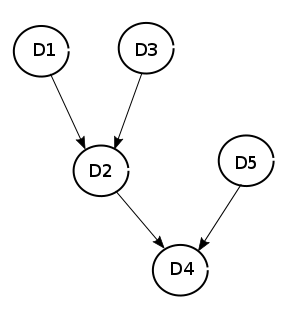
\includegraphics[width=0.4\textwidth]{grafos.png}
	\caption{Παράδειγμα Γράφου προτεραιότητας}
\end{figure}

\begin{lstlisting}[caption={Εντολές παραλληλισμού του παραπάνω παραδείγματος}]
cobegin
	begin
		cobegin
		D1;
		D3;
		coend;
		D2;
	end;
	D5;
coend;
D4;
\end{lstlisting}

\subsubsection{Συγχρονισμός} 


\paragraph{Κρίσιμες περιοχές - Αμοιβαίος αποκλεισμός}

\begin{itemize}
	\item 	Κρίσιμη περιοχή: Η περιοχή που περιέχει προσπελάσεις σε
		διαμοιραζόμενες περιοχές μνήμης ή αρχεία
	\item	Επιθυμητός ο αμοιβαίος αποκλεισμός: αποκλεισμός μιας
		διεργασίας από κάποια ενέργεια που ταυτόχρονα επιτελεί
		κάποια άλλη διεργασία
	\item	Λύση: Συγχρονισμός που προϋποθέτει τις ακόλουθες
		συνθήκες:
		\begin{enumerate}
			\item	Δυο διεργασίες δεν βρίσκονται ποτέ ταυτόχρονα στα κρίσιμα τμήματά
				τους (αμοιβαίος αποκλεισμός).
			\item	Δεν επιτρέπονται υποθέσεις σε ό,τι αφορά την ταχύτητα ή το πλήθος
				των επεξεργαστών.
			\item	Διεργασία που δεν βρίσκεται σε κρίσιμο τμήμα δεν επιτρέπεται να
				αναστείλει άλλες διεργασίες (progress).
			\item	Δεν επιτρέπεται η επ’ αόριστον αναμονή μιας διεργασίας για να
				εισέλθει στο κρίσιμο τμήμα της (bounded waiting).
		\end{enumerate}
\end{itemize}

\paragraph{Κρίσιμη περιοχή - Υλοποίηση}

\indent Πως μπορεί να υλοποιηθεί μια κρίσιμη περιοχή;
με «έξυπνες» λύσεις που βασίζονται στο λογισμικό
με τη χρήση «εργαλείων» που προσφέρουν τα ΛΣ
(αλλά και κάποιες – παλαιότερες - υψηλές γλώσσες
προγραμματισμού) όπως είναι οι σημαφόροι και οι
κρίσιμες περιοχές / κρίσιμες περιοχές υπό συνθήκη
με τη χρήση των δυνατοτήτων του hardware (π.χ. η
συνάρτηση TestAndSet)

